%----------------------------------------------------------------------------------------
%	PACKAGES AND THEMES
%----------------------------------------------------------------------------------------
\documentclass[aspectratio=169, t]{beamer}

\mode<presentation> {
\usetheme{Madrid}
\setbeamertemplate{navigation symbols}{}
}

\usepackage{graphicx}
\usepackage{booktabs}

%----------------------------------------------------------------------------------------
%	TITLE PAGE0
%----------------------------------------------------------------------------------------
\title[Electronic Hardware Design]{Electronic Hardware Design}

\author{Josh Johnson}
\date{BSides Canberra 2021}

\begin{document}
\begin{frame}
\titlepage
\end{frame}

%----------------------------------------------------------------------------------------
%	PRESENTATION SLIDES
%----------------------------------------------------------------------------------------
\begin{frame}
\frametitle{Overview}
What is a PCB?

Workflow
\begin{itemize}
	\item Requirements
	\item Locating Resources / Refrence Designs
	\item Schematic Capture
	\item Printed Circuit Board Layout
	\item Ordering PCBs / Components
	\item Assembly
\end{itemize}
Examples - LED Bow Tie
\begin{itemize}
	\item Breadboard
	\item Through Hole PCB
	\item Fully Integrated Design
\end{itemize}
\end{frame}

%----------------------------------------------------------------------------------------
\begin{frame}
	\frametitle{What is a PCB?}
	\begin{figure}
		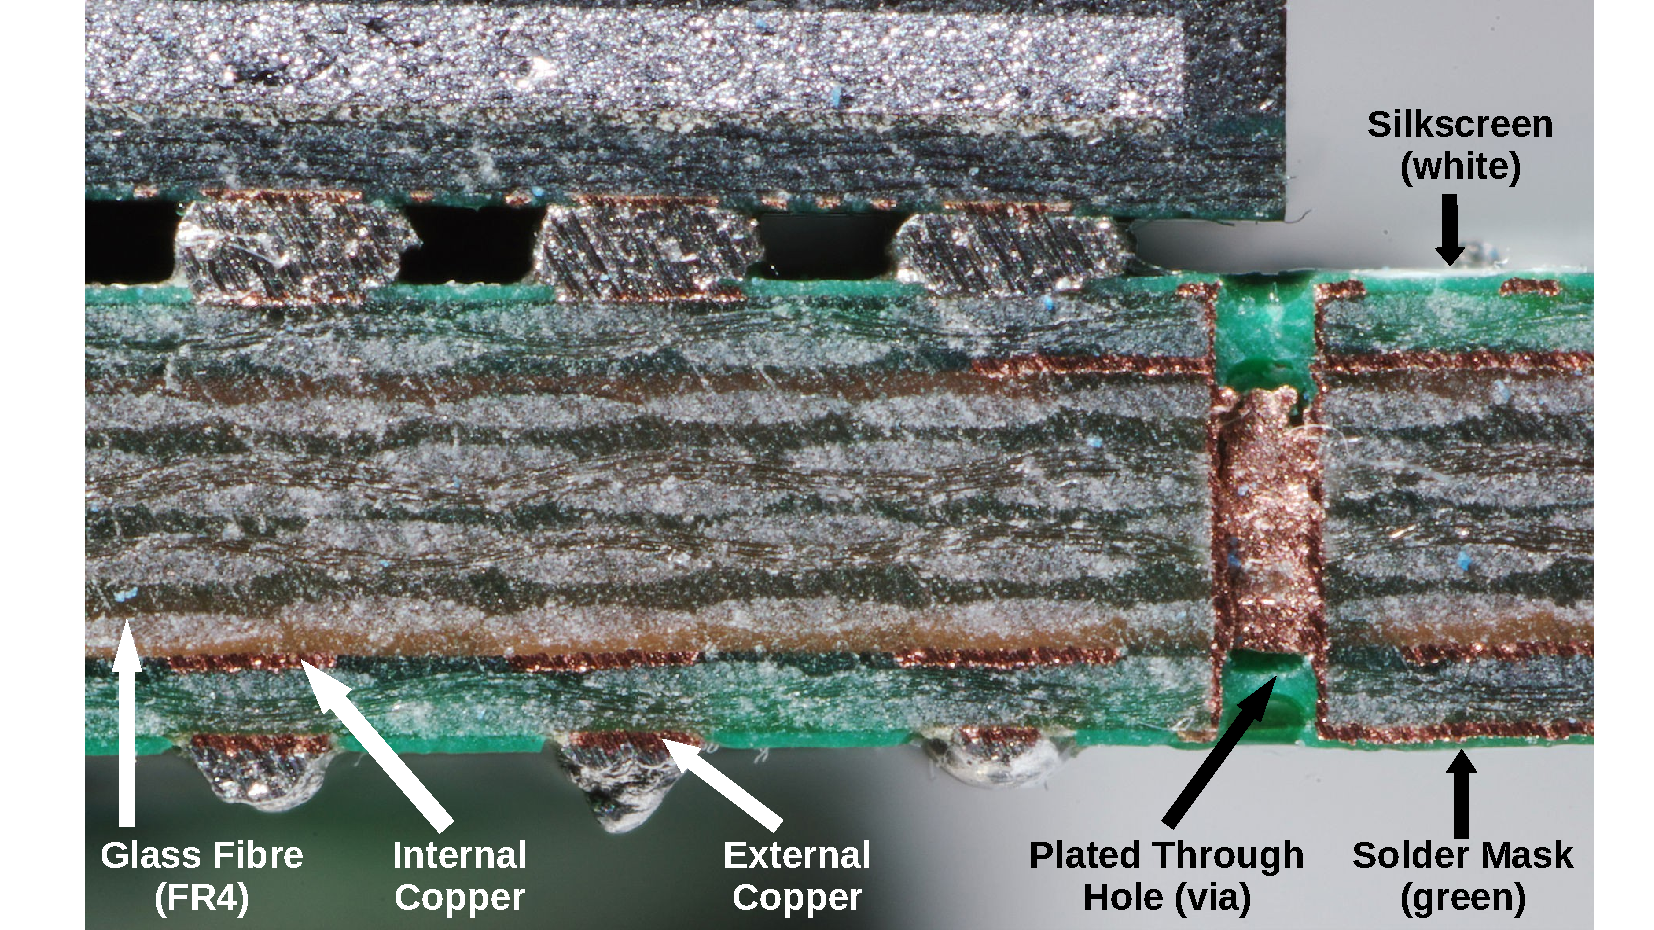
\includegraphics[width=11cm]{images/pcb-cross-section-markup.pdf}

		\text{Image: Rainer Knäpper}
	\end{figure}
\end{frame}

%----------------------------------------------------------------------------------------
\begin{frame}
\frametitle{Requirements}
Depending on the objective of your design, there are a number of requirements / considerations which need to be taken into account as they will greatly impact your finished product. \\[10pt]

\begin{itemize}
	\item Physical dimensions / form factor
	\item Interacting with design (buttons, sensors, displays, LEDs)
	\item Connectivity (USB, Bluetooth, WiFi)
	\item Programming (bootloader, on board / external programmer, Arduino / C / Python)
	\item Power supply / battery
	\item Complexity (component size, COTS modules, part count)
	\item Assembly (through hole, surface mount, single vs double sided)
	\item Cost (PCB features, component selection)
\end{itemize}
\end{frame}

%----------------------------------------------------------------------------------------
\begin{frame}
\frametitle{Locating Resources / Refrence Designs}
With requirements in hand, we can now start searching for suitable parts.\\
Evalulation boards are a great place to start, as they provide working hardware, documentation, and example code if applicable.\\[10pt]

\begin{itemize}
	\item Adafruit / Sparkfun
	\item OSHW (GitHub, Hackaday.io)
	\item Manufacturer Evaluation Boards
	\item Application Notes
	\item Datasheet
\end{itemize}
\vspace{10pt}
All of the above will provide you with schematics and part numbers to kick start your design.
\end{frame}

%----------------------------------------------------------------------------------------
\begin{frame}
\frametitle{Schematic Capture}
\begin{columns}
	\column{.6\textwidth}
	What: Abstract representation of circuit / components.\\
	Why: Communicates purpose and documents design.\\
	How:
	\begin{itemize}
		\item Symbol creation
		\item Symbol placement
		\item Connect everything with wires
		\item Add notes to your design
		\item Run electrical rules checks (ERC)
		\item Footprint association (may be done in symbol placement)
		\item Bill of Materials (BOM) generation 
	\end{itemize}
	
	\column{0.39\textwidth}
	\vspace{-8mm}
	\begin{figure}
		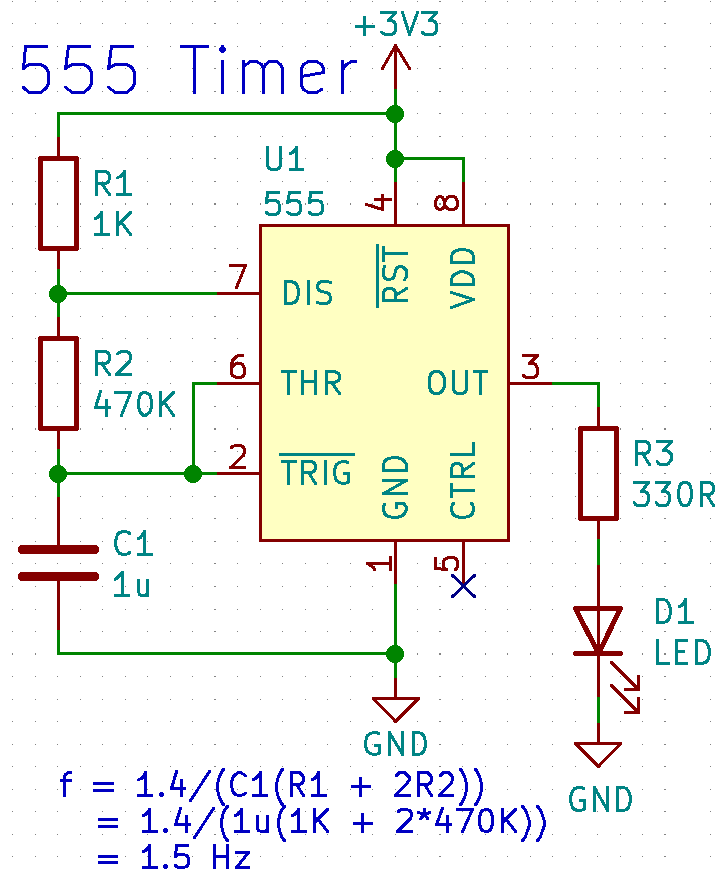
\includegraphics[width=\linewidth]{images/555-schematic-snip.png}
	\end{figure}
\end{columns}
\end{frame}

%----------------------------------------------------------------------------------------
\begin{frame}
\frametitle{PCB Layout}
\begin{columns}
	\column{.6\textwidth}
	What: Physical representation of circuit / components.\\
	Why: Ensures electrical and mechanical function.\\
	How:
	\begin{itemize}
		\item Configure design rules per manufacturer guidelines
		\item Draw board outline
		\item Place connectors and mounting holes
		\item Place electronic components
		\item Route critical nets, power, then everything else
		\item Add decorative features
		\item Review in 3D viewer / check mechanical fit
		\item Run design rule checks (DRC)
		\item Export Gerbers
	\end{itemize}
	
	\column{0.39\textwidth}
	\vspace{-7mm}
	\begin{figure}
		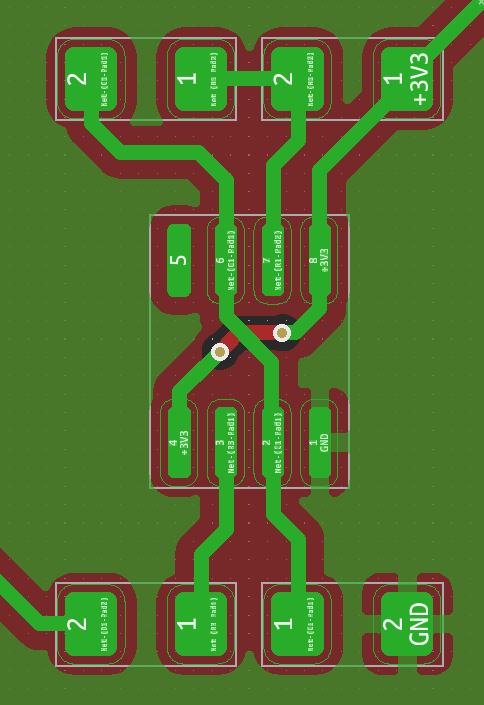
\includegraphics[width=0.8\linewidth]{images/555-layout.png}
	\end{figure}
\end{columns}
\end{frame}

%----------------------------------------------------------------------------------------
\begin{frame}
\frametitle{Ordering PCBs / Components}
\begin{columns}
	\column{.5\textwidth}
	PCB
	\begin{itemize}
		\item Check Gerbers were exported correctly
		\item Zip up Gerbers
		\item Upload to manufacturer
		\item Choose PCB options (colour, surface finish)
	\end{itemize}
	
	\column{0.49\textwidth}
	Components
	\begin{itemize}
		\item Export BOM from Schematic
		\item Upload to supplier
		\item Confirm package size is correct
	\end{itemize}
	
\end{columns}
\end{frame}

%----------------------------------------------------------------------------------------
\begin{frame}
\frametitle{Assembly}
You have all the parts, but how to put them together?
\begin{itemize}
	\item Development Boards - point to point or wired through a breadboard
	\item Through Hole - solder with a soldering iron
	\item Surface Mount - reflow with a stencil and solder paste or solder with an iron
	\item All - ask your PCB manufacturer to do it for you (even in small volumes)
\end{itemize}
\begin{figure}
	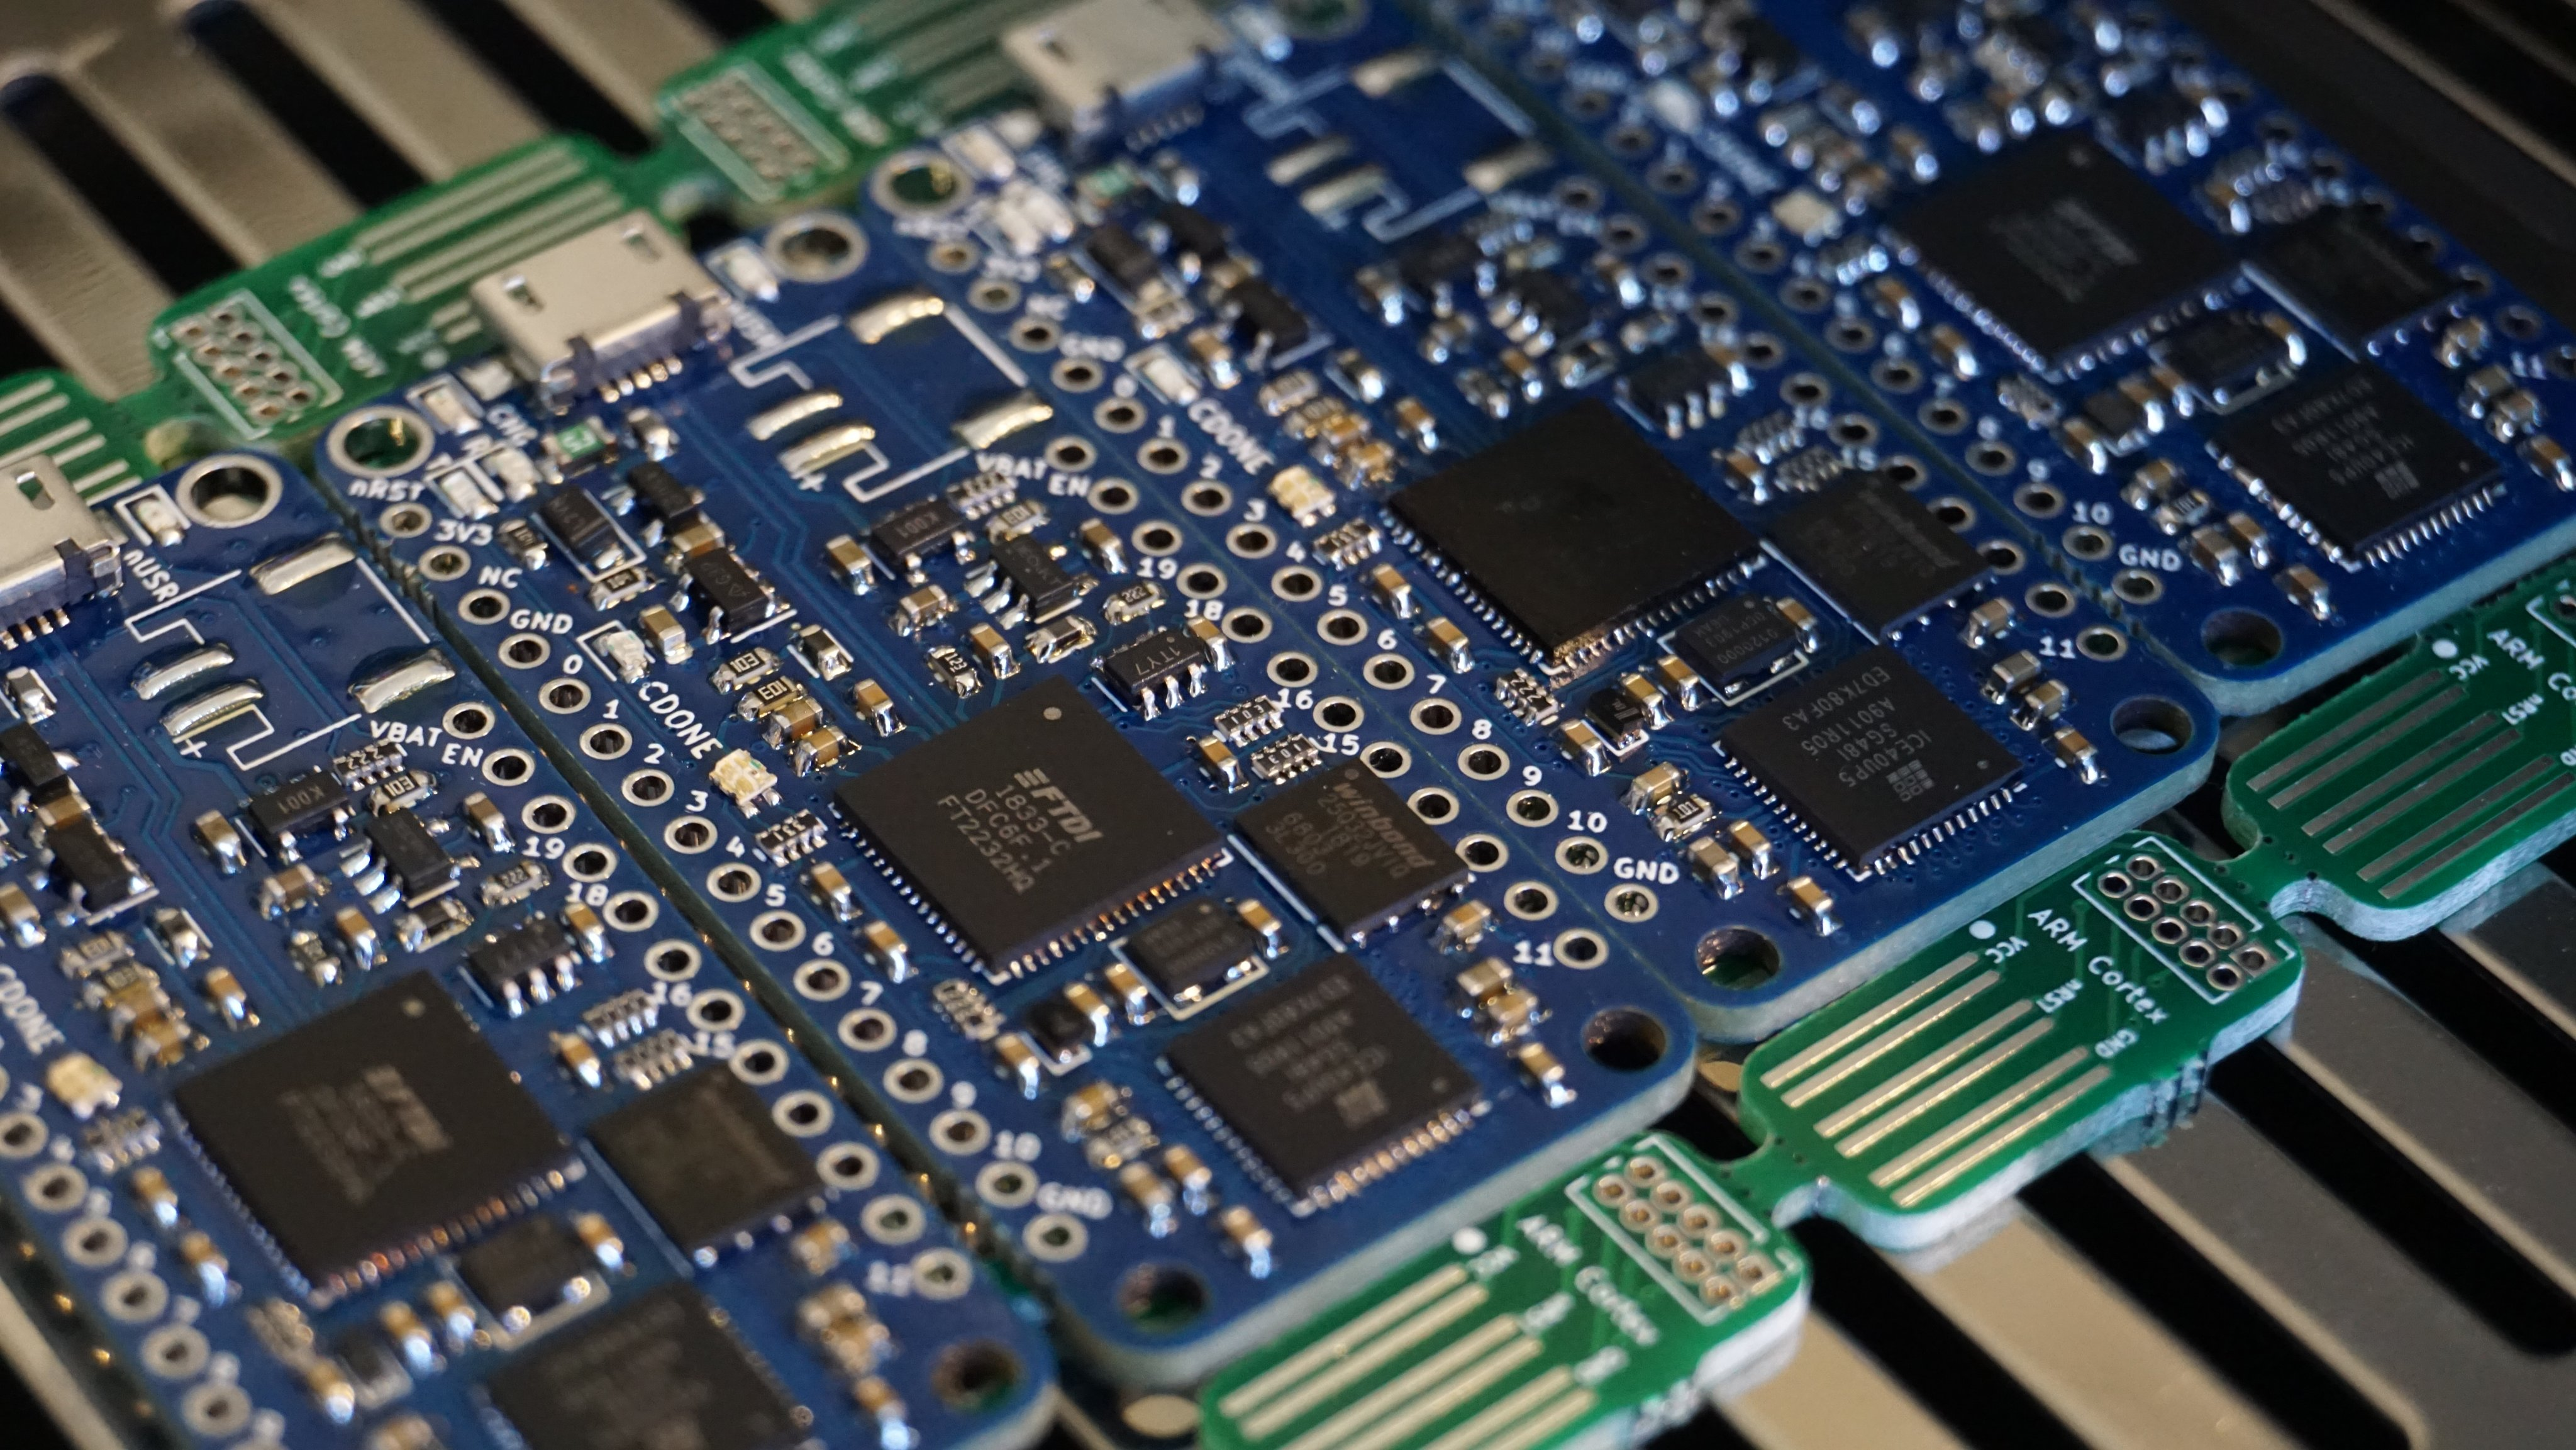
\includegraphics[height=4cm]{images/ice40-reflow.jpeg}
\end{figure}
\end{frame}

%----------------------------------------------------------------------------------------
\begin{frame}
\frametitle{Questions?}
Slides and supporting documentation: \url{github.com/joshajohnson/bsidescbr2021}\\[10pt]
README contains links if you want to learn more.\\[10pt]
I have lots of PCBs, please say hello!\\[10pt]
\vspace{5mm}

Twitter: @\textunderscore joshajohnson\\
BSidesCbr Slack: josh\\
Email: josh@joshajohnson.com\\
\vspace{4mm}
\end{frame}
\end{document} 